\documentclass{llncs}
\usepackage[utf8]{inputenc}
\usepackage[T1]{fontenc}
\usepackage[final]{graphicx}
\usepackage{epstopdf}
\usepackage[labelsep=period]{caption}
\usepackage[hyphens]{url}
\usepackage{amssymb,amsmath,mathrsfs}
\usepackage[russian,english]{babel}
\usepackage{graphicx}
\usepackage{multicol}
\usepackage[ruled,vlined,linesnumbered,algosection,algo2e]{algorithm2e}
\usepackage{algorithm}
\usepackage[noend]{algorithmic}

\tolerance=1000
\hbadness=5000
\newcommand{\const}{\mathrm{const}}
\newcommand{\tsum}{\mathop{\textstyle\sum}\limits}
\newcommand{\tprod}{\mathop{\textstyle\prod}\limits}
\newcommand{\cov}{\mathop{\rm cov}\limits}
\newcommand{\Dir}{\mathop{\rm Dir}\nolimits}
\newcommand{\norm}{\mathop{\rm norm}\limits}
\newcommand{\KL}{\mathop{\rm KL}\nolimits}
%\renewcommand{\geq}{\geqslant}
%\renewcommand{\leq}{\leqslant}
\newcommand{\eps}{\varepsilon}
\newcommand{\cond}{\mspace{3mu}{|}\mspace{3mu}}
\newcommand{\Loss}{\mathscr{L}}
\newcommand{\RR}{\mathbb{R}}
\newcommand{\cL}{\mathscr{L}}
\newcommand{\cP}{\mathscr{P}}
\newcommand{\kw}[1]{\textsf{#1}}
\SetKwFor{ForAll}{\textbf{for all}}{}{}

\begin{document}
%%Analysis of Images, Social Networks, and Texts
\title{
    BigARTM: Open Source Library for
    Regularized Multimodal %Online Parallel Distributed
    Topic Modeling of Large Collections
}
\author{
    Konstantin Vorontsov\inst{1,3,4}
    \and
    Oleksandr Frei\inst{2}
    \and
    Murat Apishev\inst{3}
    \and
    Peter Romov\inst{4}
}
\institute{
    Department of Intelligent Systems at Dorodnicyn Computing Centre of RAS,
    Moscow Institute of Physics and Technology,
    \email{voron@forecsys.ru}
    \and
    Schlumberger
    \email{...}
    \and
    Moscow State University,
    \email{...}
    \and
    Yandex
    \email{...}
}

\maketitle

\begin{abstract}
    BigARTM...

\vspace{1em}
\textbf{Keywords:}
    probabilistic topic model,
    Probabilistic Latent Sematic Analysis,
    Latent Dirichlet Allocation,
    Additive Regularization of Topic Models,
    stochastic matrix factorization,
    EM-algorithm,
    BigARTM.
\end{abstract}

\section{Introduction}

Topic modeling is a~rapidly developing branch of statistical text analysis~\cite{blei12ptm}.
Topic model reveals a~hidden thematic structure of the text collection
and finds a~compressed representation of each document by~a~set of its topics.
Such models appear to be highly useful for many applications including
information retrieval for long-text queries,
revealing research trends and research fronts,
classification, categorization, summarization and segmentation of texts.
More ideas, models and applications are outlined in the survey~\cite{daud10knowledge}.

From the statistical point of view, a~probabilistic topic model
defines each topic by a~multinomial distribution over words,
and then describes each document with a~multinomial distribution over topics.
From the optimizational point of view,
topic modeling can be considered as a~special case
of constrained approximate stochastic matrix factorization.
Learning a~factorized representation of a~text collection
is an ill-posed problem, which has an infinite set of solutions.
Then a~regularization must be used
to~impose problem-oriented restrictions
and thus to choose a~more reasonable solution.

Hundreds of models adapted to different situations are described in the literature.
For practitioners, most of them are too difficult to quickly
understand, compare, combine and embed into applications.
Then there was a~common practice to use only the simplest models such as
\emph{Probabilistic Latent Semantic Analysis}, PLSA~\cite{hofmann99plsi} and
\emph{Latent Dirichlet Allocation}, LDA~\cite{blei03latent}.
Some of the difficulties are rooted in Bayesian learning framework,
which is dominating approach in topic modeling.
Bayesian inference of each kind of model is a~unique and laborious mathematical work,
which prevents the unification and the flexible manipulation of various topic models.
Until now, there was no freely available development tools
to easily design, modify, select, and combine topic models.

In this paper we announce \textbf{the BigARTM open source project} for
parallel distributed online topic modeling of large collections,
\texttt{http://bigartm.org}.
BigARTM is released under New BSD License, which permits free commercial and non-commercial usage of the library.
The theory of BigARTM is based on non-Bayesian multicriteria approach~---
\emph{Additive Regularization of Topic Models}, ARTM~\cite{voron14dan-eng}.
In~ARTM a~topic model is learned by maximizing the~weighted sum
of the log-likelihood and additional regularization criteria.
The optimization problem is solved by a~general regularized expectation-maximization (EM) algorithm,
in which any regularization criteria or their combination can be substituted.
Many known Bayesian topic models were revisited in terms of ARTM in~\cite{voron14aist,voron14mlj}.
Compared to the Bayesian approach,
ARTM makes topic models easier to design, infer, combine and explain,
thus reducing barriers to entry into topic modeling research field.

The rest of the paper is organized as follows.
In~section~\ref{sec:Multimodal}
we~introduce a~multimodal topic model generalized for documents with multiple accompanying discrete metadata.
In~section~\ref{sec:Online}
we~describe a~fast online algorithm~\cite{hoffman10online} generalized for any additively regularized topic models.
In~section~\ref{sec:BigARTM}
we~consider the parallel architecture and implementation details of BigARTM library.
In~section~\ref{sec:Experiments}
we~report some experiments on large datasets.
In~section~\ref{sec:Conclusions}
we~discuss advantages, limitations and open problems of BigARTM.


\section{Multimodal regularized topic model}
\label{sec:Multimodal}

%Matching Words and Pictures, MoM-LDA \cite{barnard03matching}
%\cite{virtanen12factorized}
%\cite{roller13multimodal}

Let
$D$ denote a finite set (collection) of texts and
$W^1$ denote a~finite set (vocabulary) of all terms from these texts.
Each term can be a~single word or a~key phrase.
%Each document ${d\in D}$ is a sequence of terms from the vocabulary~$W^1$.
Denote $n_{dw}$ the number of times the term~$w$ appears in the document~$d$.
A document can contain not only words, but also elements of other modalities, which we also call terms.
Each $m$-th modality is defined by the finite set (vocabulary) of its terms $W^m$, ${m=1,\dots,M}$.
Examples of not-word modalities are:
authors,
class or category labels,
date-time stamps,
references to or from other documents,
entities mentioned in texts,
objects found in the images illustrating texts,
users that read or downloaded documents,
advertising banners,
etc.

Following the idea of Correspondence LDA~\cite{blei03modeling}
and Dependency LDA~\cite{rubin12statistical}
we introduce the topic model of each $m$-th modality:
\[
    p(w\cond d)
    = \sum_{t\in T} p(w\cond t)\: p(t\cond d)
    = \sum_{t\in T} \phi_{wt} \theta_{td},
    \quad
    d\in D,\; w\in W^m,\; m=1,\dots,M.
\]

The model parameters
$\phi_{wt}=p(w\cond t)$ and $\theta_{td}=p(t\cond d)$
form the matrices
$\Phi^m = \bigl( \phi_{wt} \bigr)_{W^m\times T}$ of \emph{term probabilities for the topics}, and
$\Theta = \bigl( \theta_{td} \bigr)_{T\times D}$ of \emph{topic probabilities for the documents}.
Matrices $\Phi^m$, if stacked vertically,
form ${W\!\!\times\!T}$-matrix~$\Phi$,
where ${W=W^1\sqcup\cdots\sqcup W^m}$ is disjoint union of all modalities.
Matrices $\Phi^m$ and~$\Theta$ are \emph{stochastic},
that is, their columns $\phi^m_t$, $\theta_d$
are non-negative and normalized representing discrete distributions.
The number of topics~$|T|$ is usually assumed to be
much smaller than~$|D|$ and some of~modalities~$|W^m|$.

To learn parameters $\Phi^m$, $\Theta$ from the multimodal text collection
we maximize the log-likelihood for $m$-th modality:
\[
    \cL_m (\Phi^m,\Theta) =
    \sum_{d\in D}\sum_{w\in W^m} n_{dw} \ln p(w\cond d)
    \to \max_{\Phi^m,\Theta},
\]
where
$n_{dw}$ is the number of occurrences of the term $w\in W^m$ in the document~$d$.
Note that topic distributions of documents $\Theta$ are common for all modalities.
Following the ARTM approach,
we add a~regularization penalty term $R(\Phi,\Theta)$
and solve the constrained multicriteria optimization problem via scalarization:
\begin{gather}
\label{eq:multimodal}
    \sum_{m=1}^M \tau_m \cL_m (\Phi^m,\Theta)
    + R(\Phi,\Theta)
    \to \max_{\Phi,\Theta};
\\\label{eq:multimodal:norm}
    \sum_{w\in W^m}\!\!\! \phi_{wt} = 1,~
    \phi_{wt}\geq 0;
    \qquad
    \sum_{t\in T} \theta_{td} = 1,~
    \theta_{td}\geq 0.
\end{gather}

\begin{theorem}
\label{th:multimodal}
    If the function $R(\Phi,\Theta)$ is continuously differentiable
    then the local maximum $(\Phi,\Theta)$
    of the problem~\eqref{eq:multimodal},~\eqref{eq:multimodal:norm}
    satisfies the system of equations
    with auxiliary variables $p_{tdw} = p(t\cond d,w)$:
    \begin{align}
        \label{eq:Estep}
        p_{tdw} &= \norm_{t\in T} \bigl(\phi_{wt}\theta_{td}\bigr);
    \\
        \label{eq:Mstep:phi}
        \phi_{wt} &= \norm_{w\in W^m}
            \biggl(
                n_{wt} + \phi_{wt} \frac{\partial R}{\partial \phi_{wt}}
            \biggr);
        \quad
        n_{wt} = \sum_{d\in D} n_{dw} p_{tdw};
    \\
        \label{eq:Mstep:theta}
        \theta_{td} &= \norm_{t\in T}
            \biggl(
                n_{td} + \theta_{td} \frac{\partial R}{\partial \theta_{td}}
            \biggr);
        \quad
        n_{td} =
            \sum_{w\in d} \tau_{m(w)} n_{dw} p_{tdw};
            %\sum_{m=1}^M \tau_m \!\!\sum_{w\in W^m}\!\!\! n_{dw} p_{tdw};
    \end{align}
    where
    $\norm_{t\in T} x_t = \frac{\max\{x_t,0\}}{\sum\limits_{s\in T} \max\{x_s,0\}}$
    transforms a~vector $(x_t)_{t\in T}$ to a~discrete distribution;
    $m(w)$~is the modality of the term~$w$, so that $w\in W^{m(w)}$.
\end{theorem}

This statement follows from Karush--Kuhn--Tucker conditions.
The system of equations can be~solved by various numerical methods.
Particularly,
the simple-iteration method is equivalent to the EM algorithm,
which is typically used in~practice.
For single modality (${M=1}$) Theorem~1 gives the regularized EM algorithm~\cite{voron14aist,voron14mlj}.
Many Bayesian topic models can be considered as its special cases with different regularizers~$R$.
For example,
LDA~\cite{blei03latent} corresponds to the entropy smoothing regularizer.
PLSA~\cite{hofmann99plsi} has no regularization at all, ${R=0}$.

\section{Online topic modeling}
\label{sec:Online}
%\cite{zhang13sparse}

Following the idea of Online LDA \cite{hoffman10online}
we split the collection~$D$ into batches~$D_b$, ${b=1,\dots,B}$,
and organize EM iterations so that
each document vector $\theta_d$ is~iterated until convergence at a~constant matrix~$\Phi$,
see Algorithm~\ref{alg:Online} and~\ref{alg:ProcessBatch}.
Matrix~$\Phi$ is updated rarely, after all documents from the batch are processed.
For a~large collection,
matrix~$\Phi$ stabilizes after a~small initial part of the collection passed.
Therefore a~single pass through the collection is usually sufficient to learn a~topic model
(with possible second pass for only the initial part).

Algorithm~\ref{alg:Online} does not specify how often to synchronize $\Phi$ matrix at step \ref{alg:sync}.
It can be done after every batch or less frequently
(for instance if $\frac{\partial R}{\partial \phi_{wt}}$ takes long time to evaluate).
This flexibility is especially important for concurrent implementation of the algorithm,
where multiple batches are processed in parallel.
In this case synchronization can be triggered when a fixed number of documents had been processed since last synchronization.

Such online reorganization of the EM iterative process
is not necessarily associated with Bayesian inference presented in~\cite{hoffman10online}.
Different topic models from PLSA to multimodal and regularized models
can be learned by the above online implementation of the EM algorithm.

\begin{algorithm}[t]
\caption{~Online EM-algorithm for multimodal ARTM}
\label{alg:Online}
\begin{algorithmic}[1]
\REQUIRE collection $D_b$, discounting factor $\rho$;
\ENSURE matrix $\Phi$;
\STATE initialize $\phi_{wt}$ for all $w \in W$ and $t \in T$;
\STATE $n_{wt} := 0$,~ $\tilde n_{wt} := 0$;
\FORALL{batches $D_b$, $b = 1,\dots,B$}
    \STATE $\tilde n_{wt} := \tilde n_{wt} + \kw{ProcessBatch}(D_b, \phi_{wt})$;
    \IF{(synchronize)} \label{alg:sync}
        %\STATE $n_{wt} := \kw{Merge} (n_{wt}, \tilde n_{dw})$;
        %\STATE $r_{wt} := \kw{Regularize} (n_{wt})$;
        %\STATE $n_t := \sum_{w \in W} max(0, n_{wt} + r_{wt})$;
        \STATE \label{alg:merging}
               $n_{wt} := \rho n_{wt} + \tilde n_{dw}$ for all $w \in W$ and $t \in T$;
        \STATE \label{alg:phi}
               $\phi_{wt} := \norm_{w\in W^m}
                    \bigl(
                        n_{wt} + \phi_{wt} \frac{\partial R}{\partial \phi_{wt}}
                    \bigr)$ for all $w \in W$ and $t \in T$;
        \STATE $\tilde n_{wt} := 0$ for all $w \in W$ and $t \in T$;
    \ENDIF
\ENDFOR
\end{algorithmic}
\end{algorithm}

\begin{algorithm}[t]
\caption{~$\kw{ProcessBatch} (D_b, \phi_{wt})$}
\label{alg:ProcessBatch}
\begin{algorithmic}[1]
\REQUIRE batch $D_b$, matrix $\phi_{wt}$;
\ENSURE matrix $\tilde n_{wt}$;
\STATE $\tilde n_{wt} := 0$ for all $w \in W$ and $t \in T$;
\FORALL{ $d \in D_b$}
	\STATE initialize $\theta_{td} := \frac{1}{|T|}$ for all $t \in T$;
	\REPEAT
        \STATE $p_{tdw} := \norm_{t\in T} \bigl(\phi_{wt}\theta_{td}\bigr)$ for all $t \in T$;
        \STATE $n_{td} := \sum_{w\in d} \tau_{m(w)} n_{dw} p_{tdw}$ for all $t \in T$;
        \STATE $\theta_{td} := \norm_{t\in T}
                    \bigl(
                        n_{td} + \theta_{td} \frac{\partial R}{\partial \theta_{td}}
                    \bigr)$ for all $t \in T$;
	\UNTIL{$\theta_d$ converges};
	\STATE increment $\tilde n_{wt}$ by $n_{dw} p_{tdw}$ for all $w \in d$ and $t \in T$;
\ENDFOR
\end{algorithmic}
\end{algorithm}


\section{BigARTM architecture}
\label{sec:BigARTM}

The main goal for BigARTM architecture is to ensure constant memory usage regardless of the size of the collection.
For this reason each $D_b$ batch should be stored on disk in a separate file,
and only a limited number of batches will be loaded into the main memory at any given time.
The entire $\Theta$ matrix is also never stored in the memory.
As the result, the memory usage stays constant regardless of the size of the collection.

\paragraph{Concurrency.}
An general rule of concurrency design is to express parallelism at the highest possible level.
For this reason BigARTM goes for concurrent processing of the batches
and keeps a single-threaded code for the $\kw{ProcessBatch}(D_b, \phi_{wt})$ routine.

\begin{figure}[h!]
\begin{centering}
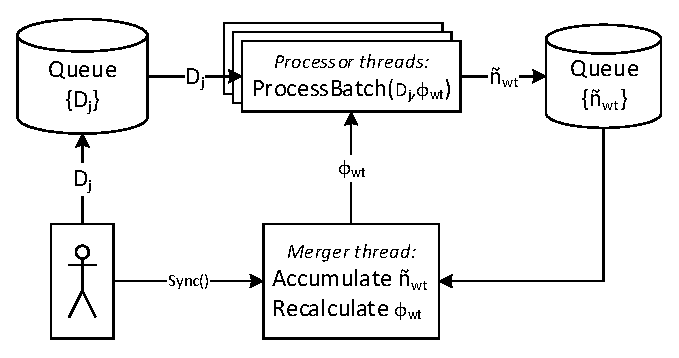
\includegraphics[height=40mm]{diagramm_artm_core.eps}
\caption{Diagram of key BigARTM components}
\label{fig:diagramm_artm_core}
\end{centering}
\end{figure}

To run multiple $\kw{ProcessBatch}$ in parallel the inputs and outputs of this routine are stored in two separate in-memory queues,
locked for push and pop operations with spin locks.
This approach does not add any noticeable synchronization overhead because
both queues only store smart pointers to the actual data objects,
so push and pop operations does not involve copying or relocating big objects in the memory.

Smart pointers are also essential for handling of the $\phi_{wt}$ matrix.
This matrix is \emph{read} by all processors threads, and can be \emph{written} at any time by the merger thread.
To resolve this conflict we keep two copies of the $\phi_{wt}$~--- an \emph{active $\Phi$} and a \emph{background $\Phi$} matrices.
The active matrix is read-only, and is used by the processor threads.
The background matrix is being built in a background by the merger thread
at steps \ref{alg:merging} and~\ref{alg:phi} of Algorithm~\ref{alg:Online},
and once it is ready merger thread marks it as active.
Before processing a new batch the processor thread gets the current active matrix from the merger thread.
This object is passed via shared smart pointer to ensure that processor thread can keep ownership of the $\phi_{wt}$ matrix
until the batch is fully processed.

Note that all processor threads share the same $\Phi$ matrix,
which means that memory usage stays at constant level regardless of how many cores are used for computation.
Using memory for two copies of the $\Phi$ matrix in our opinion gives a reasonable usage balance between memory and CPU resources.
An~alternative solution with only one $\Phi$ matrix is also possible, but it would require a heavy usage of atomic CPU instructions.
Such operations are very efficient, but still come at a considerable synchronization cost%
\footnote{\url{http://stackoverflow.com/questions/2538070/atomic-operation-cost}},
and using them for all reads and writes of the $\Phi$ matrix would cause a significant performance degradation for merger and processor threads.
Besides, an arbitrary overlap between reads and writes of the $\Phi$ matrix eliminates any possibility of producing a deterministic result.
The design with two copies of the $\Phi$ matrix gives much more control over this
and in certain cases allows BigARTM to behave in a fully deterministic way.

The design with two $\Phi$ matrices only supports a~single merger thread,
and we believe it should cape with all $n_{wt}$ updates coming from many threads.
This is a reasonable assumption because
merging at step~\ref{alg:merging} takes only about $O(|W|\cdot|T|)$ operations to execute, while
$\kw{ProcessBatch}$ takes $O(n |T| I)$ operations,
where
$n$~is the number of non-zero entries in the batch,
$I$~is the average number of inner iterations in $\kw{ProcessBatch}$ routine.
The ratio $n / |W|$ is typically from 100 to 1000 (based on datasets in UCI Bag-Of-Words repository),
and $I$ is $10 \dots 20$, so the ratio safely exceeds the expected number of cores
(up to 32 physical CPU cores in modern workstations, and even 60 cores if we are talking about Intel Xeon Phi co-processors).

\paragraph{Data layout.}
BigARTM uses dense single-precision matrices to represent $\Phi$ and $\Theta$.
Together with the $\Phi$ matrix we store a global dictionary for all words $w \in W$.
This dictionary is implemented as $\kw{std::unordered\_map}$ that maps a string representation of $w \in W$
into its integer index in the $\Phi$ matrix.
This dictionary can be extended automatically as more and more batches came through the system.
To achieve this each batch $D_b$ always has a local dictionary $W_b$, listing all words that occur in the batch.
The $n_{dw}$ elements of the batch are stored as a sparse CSR matrix (Compressed Sparse Raw format),
where each row correspond to a document $d \in D_b$, and words $w$ run over a local batch dictionary $W_b$.

For performance reasons $\Phi$ matrix is stored in column-major order, and $\Theta$ in row-major order.
This layout ensures that $\sum_t \phi_{wt} \theta_{td}$ sum runs on sequential memory elements.
In both matrices all values smaller than $10^{-16}$ are always replaced with zero to avoid performance issues with denormalized numbers
\footnote{\url{http://en.wikipedia.org/wiki/Denormal_number#Performance_issues}}.
%http://stackoverflow.com/questions/9314534/why-does-changing-0-1f-to-0-slow-down-performance-by-10x

\paragraph{Programming interface.}
All functionality of BigARTM is expressed in a set of $\kw{extern C}$ methods,
To input and output complex data structures this API uses Google Protocol Buffers
\footnote{\url{http://code.google.com/p/protobuf/}}.
This approach makes it easy to integrate BigARTM into almost any research or production environment,
because almost every modern language has an implementation of Google Protocol Buffers
and a way of calling $\kw{extern C}$ code
(``ctypes'' module for Python, ``loadlibrary'' for Matlab, ``PInvoke'' for C\#, etc).

On top of the $\kw{extern C}$ API BigARTM already has convenient wrappers in C++ and Python.
We are also planning to implement a Java wrapper in the near future.

In addition to the programming APIs the library also also has a simple CLI interface.

\paragraph{Basic tools.}
Most of BigARTM code is written in C++,
and can be built on various operating systems (Windows, Linux, and Mac OS-X)
in both 32 bit and 64 bit configurations.
To build the the library you need a recent C++ compiler with C++11 support (GNU GCC 4.6.3, clang 3.4 or Visual Studio 2012 or newer),
and Boost C++ Libraries (version 1.46.1 or newer).
All other third-parties are included in BigARTM repository:
\begin{itemize}
\item Google Protocol Buffers,
\item Google C++ Testing Framework (gtest),
\item Google Logging library for C++ (glog),
\item Google Commandline flags module for C++ (gflags),
\item ZeroMQ (\url{http://zeromq.org/}),
\item rpcz (\url{http://code.google.com/p/rpcz/}).
\end{itemize}
We also use several free online services to host this project:
\begin{itemize}
\item \url{https://github.com/bigartm/bigartm} --- to host source code,
\item \url{https://readthedocs.org/} --- free documentation hosting,
\item \url{http://travis-ci.org} --- free continuous integration service.
\end{itemize}

\section{Experiments}
\label{sec:Experiments}

\section{Conclusions}
\label{sec:Conclusions}

BigARTM architecture has a rich potential.
Current components can be reused in a distributed solution that runs on cluster.
Further improvement of single-node can be achieved by offloading batch processing into GPU.

\bigskip
\subsubsection*{Acknowledgements.}
    The work was supported by~the Russian Foundation for Basic Research grants 14-07-00847, 14-07-00908,
    and by~Skolkovo Institute of Science and Technology (project 081-R).



%%%%%%%%%%%%%%%%%%%%%%%%%%%%%%%%%%%%%%%%%%%%%%%%%%%%%%%%%%%%%%%%%%%%%%%%%%%%
%\def\BibUrl#1.{\relax}
%\bibliographystyle{gost71sv}
\bibliographystyle{splncs}
\bibliography{MachLearn}
%%%%%%%%%%%%%%%%%%%%%%%%%%%%%%%%%%%%%%%%%%%%%%%%%%%%%%%%%%%%%%%%%%%%%%%%%%%%


\end{document}

